%%%%%%%%%%%%%%%%%%%%%%%%%%%%%%%%%%%%%%%%%%%%%%%%%%%%%%%%%%%%%%%%%%%
%%%%%%%%%%%%%%%%%%%%%%%%%%%%%%%%%%%%%%%%%%%%%%%%%%%%%%%%%%%%%%%%%%%
%%%%%%%%%%%%%%%%%%%%%%%%%%%%%%%%%%%%%%%%%%%%%%%%%%%%%%%%%%%%%%%%%%%
\begin{frame}
  \frametitle{Kokkos Concepts (1) - the abstract machine model}

  \begin{itemize}
  \item Kokkos defines an abstract machine model for future large shared-memory nodes made of
    \begin{itemize}
    \item \textcolor{blue}{\bf latency-oriented cores} (multicore CPU)
    \item \textcolor{orange}{\bf throughput-oriented cores} (GPU, ...)
    \end{itemize}
  \end{itemize}

  \begin{center}
    \begin{figure}
      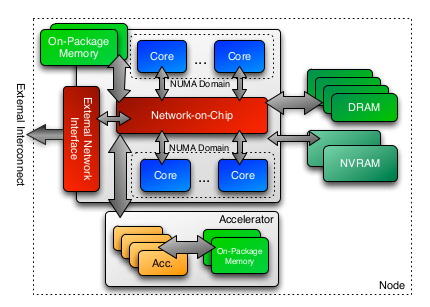
\includegraphics[width=4.5cm]{images/kokkos_machine_model}
      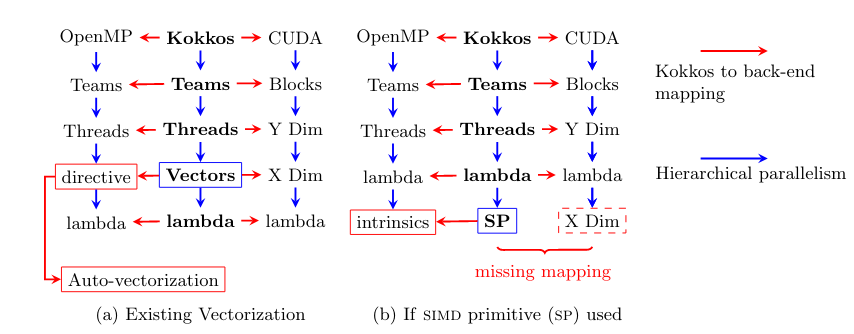
\includegraphics[width=5.5cm]{images/kokkos_simd}
      \caption{(left) Conceptual model of a current/future \textcolor{darkgreen}{\bf HPC node}. (Kokkos User's Guide).\\ (right) Abstractions mapping.}
    \end{figure}
  \end{center}
  {\small
     reference : \myhref{https://www.osti.gov/servlets/purl/1643357}{A portable SIMD primitive in Kokkos for heterogeneous architectures}}

\end{frame}


%%%%%%%%%%%%%%%%%%%%%%%%%%%%%%%%%%%%%%%%%%%%%%%%%%%%%%%%%%%%%%%%%%%
%%%%%%%%%%%%%%%%%%%%%%%%%%%%%%%%%%%%%%%%%%%%%%%%%%%%%%%%%%%%%%%%%%%
%%%%%%%%%%%%%%%%%%%%%%%%%%%%%%%%%%%%%%%%%%%%%%%%%%%%%%%%%%%%%%%%%%%
\begin{frame}[fragile=singleslide]
  \frametitle{Kokkos Concepts (2) - What is a device ?}

  \begin{itemize}
  \item Kokkos defines several {\bf c++ class} for representing a \textcolor{red}{device} in \texttt{core/src}, e.g.
    \begin{itemize}
    \item {\tt Kokkos::Cuda}, {\tt Kokkos::HIP}, {\tt Kokkos::SYCL}, {\tt Kokkos::OpenMPTarget} {\tt Kokkos::OpenMP}, {\tt Kokkos::Threads}, {\tt Kokkos::Serial}
    \item \textcolor{red}{\bf device = execution space + memory space}
    \end{itemize}
  \item Each \textit{Kokkos device} pre-defines some types
  \item Example \textcolor{red}{\textbf{Kokkos exec space}} (not required for a user, only Kokkos developper), e.g.\\
    {\tiny
      \begin{minted}{c++}
        class Cuda {
          public:
          // Tag this class as a kokkos execution space
          using execution_space = Cuda;

          #if defined( KOKKOS_USE_CUDA_UVM )
          // This execution space's preferred memory space.
          using memory_space = CudaUVMSpace;
          #else
          // This execution space's preferred memory space.
          using memory_space = CudaSpace;
          #endif

          // This execution space preferred device_type
          using device_type = Kokkos::Device<execution_space,memory_space>;

          // The size_type best suited for this execution space.
          using size_type = memory_space::size_type;

          // This execution space's preferred array layout.
          using array_layout = LayoutLeft;
          ...
        } // end class Cuda
      \end{minted}
    }
  \end{itemize}

\end{frame}

%%%%%%%%%%%%%%%%%%%%%%%%%%%%%%%%%%%%%%%%%%%%%%%%%%%%%%%%%%%%%%%%%%%
%%%%%%%%%%%%%%%%%%%%%%%%%%%%%%%%%%%%%%%%%%%%%%%%%%%%%%%%%%%%%%%%%%%
%%%%%%%%%%%%%%%%%%%%%%%%%%%%%%%%%%%%%%%%%%%%%%%%%%%%%%%%%%%%%%%%%%%
\begin{frame}
  \frametitle{Kokkos Concepts (3) - execution space, memory space}

  \begin{itemize}
  \item \textcolor{blue}{\textbf{Execution space:}} Where should a parallel contruct (\texttt{parallel\_for}, \texttt{parallel\_reduce}, ...) be executed\\
    \begin{itemize}
    \item Special case: \texttt{class HostSpace}, special device (always defined) where execution space is either (Serial, Pthread or OpenMP).
    \item Each execution space is equipped with a \texttt{fence}: \texttt{Kokkos::Cuda::fence()}
    \end{itemize}
  \item \textcolor{blue}{\textbf{Memory space:}} Where / how data are allocated in memory (HostSpace, CudaSpace, CudaUVMSpace, CudaHostPinnedSpace, HBWSpace, ...)
  \item \textcolor{blue}{\textbf{Memory layout}} (we will come back later on that)
  \item Other concepts:
    \begin{itemize}
    \item Execution policy: used to modify a parallel thread dispatch
    \end{itemize}
  \item \textcolor{red}{\bf Multiple execution / memory space} can be used in a single application\\
    See for example in Kokkos sources \texttt{example/tutorial/Advanced\_View/07\_Overlapping\_DeepCopy}\\
    Cuda stream can be used Kokkos; they must be created before {\tt Kokkos::Cuda} exec space
%meanwhile Cuda streams can be used directly (but looses some portability);~\footnote{\myhref{https://github.com/kokkos/kokkos/issues/1723}{kokkos/issues/1723}}
  \end{itemize}

\end{frame}
